\documentclass[12pt, a4paper, showtrims]{article}
\usepackage{geometry}
\usepackage{ragged2e}
\usepackage{graphicx}
\usepackage{wrapfig}
\usepackage{csvsimple}
\usepackage[utf8]{inputenc}
\usepackage{amsmath}

\graphicspath{ {./graphics/} }
\geometry{a4paper, top=2cm, bottom=2cm, hmargin=2.3cm,  includehead, includefoot}

\begin{document}
    \title{Emek Ekonomisi Ödev-1 Çözümleri}
    \author{Yasemin Hayırlı}
    \date{14 Aralık 2020}
    \maketitle

    \subsection*{Bölüm A}
    \setlength{\parindent}{0em}
    \setlength{\parskip}{0.3em}

        \subparagraph{Kukla Değişkenler} 
        \begin{justify}
        \setlength{\parindent}{0em}

Kukla değişkenler, regresyon analizinde bağımsız değişkenlerin
kategorik olarak gösterimini sağlar ve n adet kukla değişkenden bir tanesi 
referans alınarak kukla değişkenler arasında karşılaştırma yapılır. \par

Angrist ve Krueger(1991) yaptıkları çalışmada doğum çeyreklerini kukla 
değişken olarak kullanmışlardır. Doğum çeyreklerini 4 adet tanımladıklarından 
dolayı n-1 tane yani 3 adet kukla değişken oluşturulmalıdır. \par

Aşağıdaki regresyon denklemi 1920-1929 yılları için doğum çeyreklerinin 
eğitim seviyeleri üzerindeki etkisini tahmin etmektedir. Dördüncü doğum çeyreği 
referans olarak alınmış ve 3 adet kukla değişken oluşturulmuştur. 
Regresyon sonuçları Tablo 1'de gösterilmektedir.

\[ EDUC_{ij} = \alpha + \sum_{j}^{3}\beta_jQOB_{ij} + \epsilon_{ij}  \]

\begin{table}[h!]
    \centering
    \caption{Doğum Çeyreklerinin Eğitim Seviyesi Üzerindeki Etkisi}
    \begin{tabular}{||c c c c||}    
    \hline
    Sonuç Değişkeni & 1.Doğum Çeyreği & 2.Doğum Çeyreği & 3.Doğum Çeyreği \\ [0.5ex] 
    \hline\hline
    Eğitim Seviyesi & -0.151***       & -0.0947***      &  -0.0340* \\ 
                    & (0.0163)        & (0.0164)        & (0.0160)  \\
    \hline
    \multicolumn{4}{|c|}{Standart hatalar parantez içinde verilmiştir. * p<0.05, ** p<0.01, *** p<0.001} \\
    \hline
    \hline
    \end{tabular}
    
    \label{Tablo:1}
\end{table}

\subparagraph{1970 ve 1980 CENSUS'ları İçin Wald Tahminleri} 
\setlength{\parindent}{0em}    
\begin{justify}
\setlength{\parindent}{0em}     
  
    
    Eğitim süresi ile ücret arasındaki ilişkiyi gösteren Mincer Eşitliği, bireysel yeteneğin
    modele gözlemlenemediği için dahil edilememesinden dolayı seçilim yanlılığına sahiptir.
    Modeldeki seçilim yanlılığını ortadan kaldırmak için Araç Değişken (IV) Yöntemine başvurulmalıdır.
    Bir değişkenin araç değişken olarak kullabılabilmesi için seçilen araç değişken ile müdahale değişkeni
    arasında bir ilişki olması, ancak sonuç değişkeni ile ilişkisi olmaması gerekmektedir. 
    Ayrıca araç değişken tesadüfi olarak meydana gelmiş olmalıdır. \par 
    
    \newpage
    Angrist ve Krueger(1991) ABD'de yürürlükte olan okula başlama yaşı politikasından
    hareketle eğitim ile ücret arasındaki ilişkiyi tahmin edebilmek için doğum çeyreklerini 
    araç değişken olarak kullanmışlardır. Doğum çeyrekleri, bireylerin aldığı eğitim süresini
    etkilemektedir. Örneğin birinci çeyrekte doğan bireyler, diğer çeyreklerde doğanlara oranla
    daha az eğitim alırken; dördüncü çeyrekte doğan bireyler daha fazla süre eğitim görmüşlerdir.
    
    Biz burada 1. çeyrekte doğan erkeklerin 1 değeri aldığı kukla değişkeni, araç değişken $(Z_i)$ olarak
    kullanmaktayız. Müdahale değişkeni olarak eğitim süresini $(EDUC_i)$, sonuç değişkeni olarak da ücretleri 
    $(LWKLYWGE_i)$ ele alacağız.

    \[Z_i=  \begin{cases} 
        1 & Q_{i}= 1 \\
        0 & Q_{i}= 2,3,4 
     \end{cases}\]

    Eğer araç değişkenimiz 1 ve 0 gibi iki farklı değer alıyorsa, Araç Değişken (IV) Tahmini [LATE]
    "Wald Yöntemi" adını alır. Wald Yöntemi sayesinde, yerel ortalama müdahale etkisini hesaplayabiliriz.
    
    Wald Tahminini elde etmek için ilk olarak müdahale değişkeni ile araç değişkeni
    arasında nasıl bir ilişki olduğunu bulmalıyız. Bunu regresyon sayesinde de yapabiliriz. 
    Fakat burada ortalama farklar cinsinden iki değişken arasındaki ilişkiyi tahmin edeceğiz.
    Bu aşama \textbf{"I.Adım"} olarak adlandırılmaktadır.

    \[\phi = E [EDUC_i | Z_i = 1] - E[EDUC_i | Z_i = 0 ]\]

    I. Adım yapıldıktan sonra araç değişkenin sonuç değişkeni üzerindeki etkisini hesaplamamız gerekmektedir.
    Bu sayede sonuç değişkeni, araç değişkenin müdahale değişkeni üzerindeki etkisinden ayrılmış olur.
    Bu aşama \textbf{"İndirgenmiş Form"} adını almaktadır. Burada iki değişken arasındaki ilişkiyi bulabilmek için 
    ortalama farklar yöntemini kullanacağız.

    \[\rho  = E [LWKLYWGE_i | Z_i = 1] - E[LWKLYWGE_i | Z_i = 0 ]\]

    İndirgenmiş Formdan elde ettiğimiz $\rho$ ile birinci aşamada bulduğumuz $\phi$ katsayısını birbirine oranlarsak 
    Wald Tahmini olan $\lambda$ 'ya ulaşabiliriz.

    \begin{equation} 
        \begin{split}
        \lambda  = \frac{\rho}{\phi} 
        = \frac{E [LWKLYWGE_i | Z_i = 1] - E[LWKLYWGE_i | Z_i = 0 ]]}{E [EDUC_i | Z_i = 1] - E[EDUC_i | Z_i = 0 ]} 
        \end{split}
    \end{equation}

    Eğitim ile ücretler arasında herhangi bir araç değişken kullanmadan hesaplayacağımız EKK modeli ise aşağıda verilmektedir.
    Ancak bu regresyon modeli seçilim yanlılığına sahiptir. 

    \[ LWKLYWGE_i = \alpha + \beta EDUC_i + \epsilon_i  \]

    \newpage
    Ortalamalar arası farklar, Wald ve EKK tahminleri Tablo 2'de gösterilmiştir.

    \begin{table}[h]
        \centering
        \caption{1920- 1929 ve 1930-1939 Döneminde Doğan Bireyler İçin Wald Tahmini}
        \begin{tabular}{|p{3cm}||p{2cm}|p{2cm}|p{6cm}|}   
            \hline
            \multicolumn{4}{|c|}{1920-1929 "CENSUS: 1970"} \\
            \hline
         \hline
                   & 1.Doğum Çeyreği & 2. 3. ve 4. Doğum Çeyreği & Ortalamalar Arasındaki Fark \\ [0.5ex] 
         \hline
          LWKLYWGE &  5.148471       &   5.15745                 &  \textbf{-0.00898**} (İndirgenmiş Form) \\ 
                   &                 &                           &      (0.00301)  \\
          EDUC     & 11.3996         &   11.52515                &  \textbf{ -0.126***} (I. Adım) \\ 
                   &                 &                           &      (0.0155)  \\ 
          Wald Tahmini &             &                           &  0.0715** \\ 
                   &                 &                           & (0.0219) \\ 
          EKK      &                 &                           &  0.0801***\\ 
                   &                 &                           & (0.000355)  \\  
        \hline
        \multicolumn{4}{|c|}{1930- 1939 "CENSUS: 1980"} \\
        \hline
        \hline
                  & 1.Doğum Çeyreği & 2. 3. ve 4. Doğum Çeyreği & Ortalamalar Arasındaki Fark \\ [0.5ex] 
        \hline
         LWKLYWGE &  5.891596       & 5.902695                  &  \textbf{-0.0111***} (İndirgenmiş Form) \\ 
                  &                 &                           & (0.00274)  \\
         EDUC     & 12.68807        & 12.79688                  &  \textbf{-0.109***} (I. Adım) \\ 
                  &                 &                           & (0.0132)  \\ 
         Wald Tahmini &             &                           &   0.102*** \\ 
                  &                 &                           & (0.0239) \\ 
         EKK      &                 &                           &  0.0709***\\ 
                  &                 &                           & (0.000339)  \\
        \hline
        \multicolumn{4}{|c|}{EKK Tahminleri, ücretlerin bağımlı değişken ve } \\
        \multicolumn{4}{|c|}
        {eğitimin bağımsız değişken olarak alınmasıyla hesaplanmıştır.} \\
        \hline
        \multicolumn{4}{|c|}
        {Wald Tahmini, IV metod kullanılarak elde edilmiştir.} \\
        \multicolumn{4}{|c|}
        {İndirgenmiş Form katsayısının birinci adımdan elde edilen katsayıya } \\ 
        \multicolumn{4}{|c|}
        {bölünmesi ile standart sapmalara ulaşılamaz.} \\
        \hline
        \multicolumn{4}{|c|}{Standart hatalar parantez içinde verilmiştir. * p<0.05, ** p<0.01, *** p<0.001} \\
        \hline
        \hline
        \end{tabular}
        
        \label{Tablo:2}
    \end{table}

    Ortalamalar arası farklar, hem eğitim hem de ücretler için 
    belirtilen tarih aralıklarında istatiksel olarak anlamlıdır.
    Yani sıfırdan farklı değer almaktadır. \textit{(Ortalamalar arası farkların
    değerleri, standart sapmalarının iki katından daha büyüktür.)}
    Ücretler açısından her iki grup arasındaki farkların her iki dönemde 
    yaklaşık \% 1 civarında olduğu görülmektedir. Birinci çeyrekte doğan bireyler,
    diğer çeyrekte doğanlardan \% 1 oranında daha düşük ücret almaktadır.
    Eğitim açısından ise 1920- 1929 döneminde birinci çeyrekte doğan bireylerin
    diğer çeyreklerde doğanlara kıyasla yaklaşık \% 12 oranında daha az eğitim aldıkları
    görülmektedir. Bu oran 1930- 1939 yılları arasında yaklaşık \% 11'dir.


    \newpage
    \subsection*{Bölüm B}
    \setlength{\parindent}{0em}
    \setlength{\parskip}{0.3em}

    \subparagraph{2SLS Tahminleri} 
    \subparagraph{Kontrol değişkenleri kullanılmamaktadır.} 
    \begin{justify}
    \setlength{\parindent}{0em}

    2SLS Yöntemi, Wald Tahminine göre daha gelişmiştir. Birden fazla araç değişken kullanabilir ve 
    modele kontrol değişkenleri ekleyebiliriz. Ancak 2SLS Yöntemi, manuel olarak hesaplandığında doğru standart
    hataları vermez. Bu yüzden 2SLS Yöntemini ekonometrik yazılımlar aracılığıyla yapmaktayız.
    2SLS yöntemini ile eğitimin ücretlere etkisini tahmin ederken, eğitim değişkeni ve araç değişkeni içsel,
    diğer kontrol değişkenlerini dışsal kabul etmekteyiz.
    
    Kontrol değişkeni kullanılmadan uygulanan EKK, 2SLS ve Wald yöntemlerinin tahminleri Tablo 3'te 
    gösterilmektedir.



    \begin{table}[h]
        \centering
        \caption{Eğitimin Ücretlere Etkisinin EKK ve 2SLS Yöntemleri Aracılığıyla Tahminleri}
        \begin{tabular}{|p{4cm}||p{2cm}|p{2cm}|p{2cm}|}   
        \hline
        \multicolumn{4}{|c|}{1920-1929 "CENSUS: 1970"} \\
         \hline
          & EKK & 2SLS & Wald \\ [0.5ex] 
         \hline
          EDUC &  0.0801***  &  0.0715**  & 0.0715** \\ & (0.000355) & (0.0219) & (0.0219)  \\ 
        \hline
        \multicolumn{4}{|c|}{1930-1939 "CENSUS: 1980"} \\
         \hline
          & EKK & 2SLS & Wald \\ [0.5ex] 
         \hline
          EDUC & 0.0709*** & 0.102***  & 0.102*** \\ & (0.000339) & (0.0239) & (0.0239)  \\ 
        \hline
        \multicolumn{4}{|c|}{Modele kontrol değişkeni dahil edilmemiştir.} \\
        \hline
        \multicolumn{4}{|c|}{Standart hatalar parantez içinde verilmiştir. * p<0.05, ** p<0.01, *** p<0.001} \\
        \hline
        
        
        \end{tabular}
    \end{table}
    
    Kontrol değişkenleri kullanılmadan yapılan 2SLS ve Wald Tahminleri aynı sonuçlar vermektedir.
    Zaten Wald Tahmini, standart hataları ile birlikte hesaplanmak isteniyorsa 2SLS Metodu tercih edilmelidir.
    EKK, 2SLS ve Wald tahminlerinin hepsi istatiksel olarak anlamlıdır. Ayrıca 2SLS Tahmini ve 
    EKK yöntemi ile tahmin edilen sonuçlar birbirlerine oldukça yakın değerler almaktadır. Fakat 
    EKK ve 2SLS tahminleri arasındaki fark anlamlı değildir.

    \newpage
    \subparagraph{Kontrol değişkenleri kullanılmaktadır.}
    \begin{justify}
        \setlength{\parindent}{0em}

    \begin{table}[h]
        \centering
        \caption{Eğitimin Ücretlere Etkisinin EKK ve 2SLS Yöntemleri Aracılığıyla Tahminleri}
        \begin{tabular}{|p{4cm}||p{2.5cm}|p{2.5cm}||p{2.5cm}|p{2.5cm}|}   
            \hline
            \multicolumn{5}{|c|}{1920-1929 "CENSUS: 1970"} \\
         \hline
          & EKK(1) & 2SLS(2) & EKK(3) & 2SLS(4) \\ [0.5ex] 
         \hline
          EDUC & 0.0774***  & 0.0819*** &0.0726***     &  0.0721  \\ 
               & (0.000356) & (0.0217)  & (0.000359)   & (0.0426) \\
          RACE &  -         &  -        &-0.311***     & -0.312*** \\ 
               &            &           &(0.00439)     & (0.0983)\\
          AGE  &  -         &  -        &0.000256      & 0.000439 \\ 
               &            &           & (0.00269)    & (0.00255)\\
          9 YOB Dummies & Anlamsız &  Anlamlı & Anlamsız& -\\
          8 REGION Dummies & Anlamlı &  Anlamlı & Anlamlı & Anlamlı\\ 

        \hline
        \multicolumn{5}{|c|}{1930-1939 "CENSUS: 1980"} \\
         \hline
          & EKK(1) & 2SLS(2) & EKK(3) & 2SLS(4) \\ [0.5ex] 
         \hline
          EDUC &  0.0693*** & 0.104*** & 0.0664***  &  0.257**  \\ 
               &  (0.000341)& (0.0248) & (0.000341) & (0.0936) \\
          RACE &  -         &  -       & -0.275***  & 0.183 \\ 
               &            &          & (0.00407)  & (0.144)\\
          AGE  &  -         &  -       & -0.00318   & 0.0159** \\ 
               &            &          & (0.00254)  & (0.00588)\\
          9 YOB Dummies & Anlamlı &  Anlamlı & Anlamlı & -\\
          8 REGION Dummies & Anlamlı &  Anlamlı & Anlamlı & Anlamsız\\ 
 
        \hline
        \multicolumn{5}{|c|}{Standart hatalar parantez içinde verilmiştir. * p<0.05, ** p<0.01, *** p<0.001} \\
        \hline
        \end{tabular}
    \end{table}     
    
    Seçilim yanlılığı barındıran EKK sonuçlarının her iki dönemde de farklı değişkenler 
    kontrol edilerek yapılan tahminlerde istatistiki olarak anlamlı olduğu görülmektedir.
    Ancak 2SLS tahminleri için bu durum geçerli değildir. Doğum yılları kukla değişkeni ve
    bölge kukla değişkenleri kontrol edilerek yapılan ölçümlerde 2SLS tahminleri anlamlıdır.
    Ancak bu tahminlerde doğum yılları ve doğum çeyrekleri birbiriyle ilişkili olduğundan 
    araç değişkenin doğruluğu zedelenir. Doğum yıllarının dahil edilmediği modellerde ise 2SLS 
    sonuçları 1920- 1929 döneminde istatistiki olarak anlamsızdır, ancak 1930- 1939 döneminde 
    anlamlıdır. 1920- 1929 döneminde 2SLS tahminleri anlamsız olduğu için çıkan sonuçlar ile 
    EKK tahminlerini karşılaştırmak doğru değildir. Ancak 1930-1939 dönemi için karşılaştırma
    yapılabilir. 1930- 1939 dönemi için eğitimin ücret üzerindeki etkisini gösteren EKK ve 2SLS tahminleri
    birbirinden oldukça uzaktır. Ayrıca söz konusu tahminlerin standart sapmaları arasındaki fark 
    anlamlı değildir. Bundan dolayı kısa regresyon modeli, uzun regresyon modeli yerine kullanılamaz.

    
    \end{justify}

    \newpage
    \subsection*{Bölüm C}
    \setlength{\parindent}{0em}
    \setlength{\parskip}{0.3em}

    \subparagraph{Zayıf Araç Değişken Problemi}  
    \begin{justify}
    \setlength{\parindent}{0em}

    2SLS Yönteminde Zayıf Araç Değişken problemini test etmek için kullanılan araç değişken ile
    müdahale değişkeni arasında regresyon modeli kurulabilir. Doğum çeyreği için 1 değerini 
    atadığımız kukla değişkeni araç değişken olarak kullanacağız.

    \begin{table}[h!]
        \centering
        \caption{Araç Değişkenin Müdahale Değişkeni Üzerindeki Etkisi}
        \begin{tabular}{|p{3cm}||p{4cm}|p{3cm}|}
        \hline \multicolumn{3}{|c|}{1920- 1929 "CENSUS 1970"} \\\hline    
        \hline EDUC & -0.126*** & (0.0155) \\ [0.5ex] 
        \hline \multicolumn{3}{|c|}{1930- 1939 "CENSUS 1980"} \\
        \hline EDUC & -0.109*** & (0.0132) \\ [0.5ex] \hline
        \hline \multicolumn{3}{|c|}{Modellerde kontrol değişkenleri kullanılmamıştır.} \\
        \hline \multicolumn{3}{|c|}{1920- 1929 "CENSUS 1970"} \\\hline
        \hline EDUC & -0.113*** & (0.0151) \\ [0.5ex] 
        \hline \multicolumn{3}{|c|}{1930- 1939 "CENSUS 1980"} \\    
        \hline EDUC & -0.100*** & (0.0130) \\ [0.5ex] \hline
        \hline \multicolumn{3}{|c|}{Modellerde kontrol değişkenleri kullanılmıştır.} \\\hline 
        \hline \multicolumn{3}{|c|}{Standart hatalar parantez içinde verilmiştir. * p<0.05, ** p<0.01, *** p<0.001} \\\hline  

        \end{tabular}
        
        \label{Tablo:1}
    \end{table}

    Araç değişkenin müdahale değişkenine etkisine dair sonuçlar yukarıda verilmiştir.
    Elde edilen sonuçlara göre araç değişken ilgili dönemlerde, hem kontrol 
    değişkeni kullanılan hem de kontrol değişkeni kullanılmayan modellerde istatistiki olarak
    anlamlıdır. Sonuç olarak 2SLS tahminlerinde kullanılan araç değişkenin gücü yüksektir. 

    \newpage
    \subsection*{Bölüm D}
    \setlength{\parindent}{0em}
    \setlength{\parskip}{0.3em}

    \subparagraph{Grafik}
    \begin{justify}
    \setlength{\parindent}{0em}

    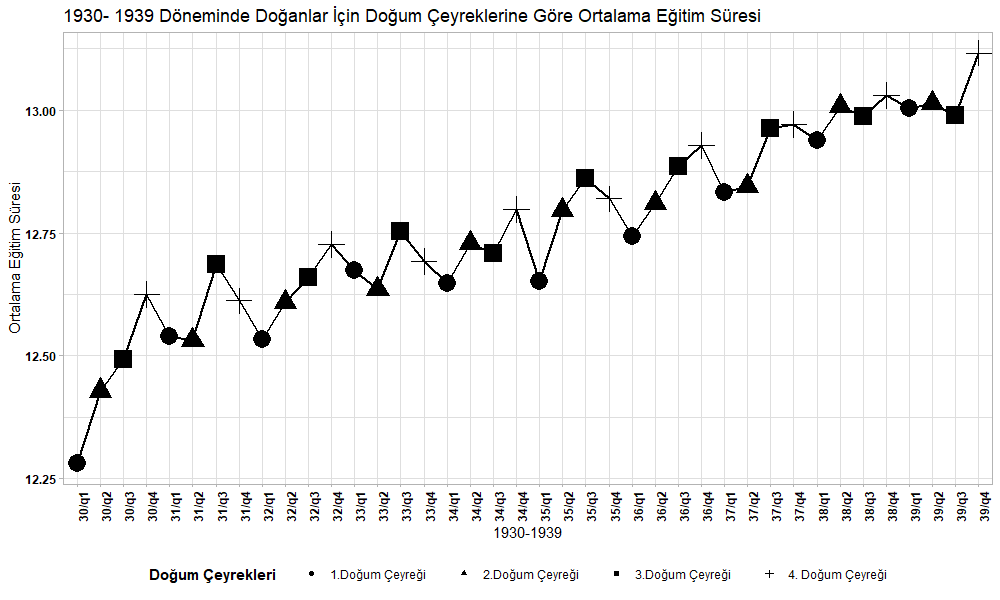
\includegraphics[width=\textwidth]{Graph.png}

    Yukarıdaki grafikte 1930- 1939 yılları arasında doğan bireylerin almış oldukları eğitim süreleri,
    doğum çeyreklerine göre ortalama olarak verilmiştir. Belirtilen tarih aralığında birinci 
    doğum çeyreğinde doğan bireyler yıllar bazında en az eğitim gören grubu oluşturmaktadır.
    En fazla eğitim gören bireyler ise üçüncü ve dördüncü çeyreklerde doğan bireylerdir.


    \end{justify}

    \end{justify}    
    \end{justify}


\end{justify}   


    
     
\end{justify}




    


\end{document}